% ClaimLoop: high-risk project report
% Compile on Overleaf with the ACM acmart class (sigconf option).
% Upload this file, claimloop.bib, and the figures/ directory.

\documentclass[sigconf,nonacm]{acmart}

\usepackage{booktabs}

\begin{document}

\title{ClaimLoop: Probing Whether LLM Agents Can Survive the Medical Claims Denial Loop}

\author{Abdullah Abdel-Khalek}
\affiliation{%
  \institution{The University of Texas at Austin}
  \city{Austin}
  \state{Texas}
  \country{USA}}
\email{abdullahhussamak@gmail.com}

\begin{abstract}
Medical claims processing is one of the costliest administrative workflows in
United States healthcare: clinical conversations must be documented, translated
into ICD-10-CM and CPT codes, assembled into claims, and defended when payers
deny them. Prior benchmarks show that large language models queried directly
for medical codes are unreliable, yet most published work stops at the coding
step and never reaches the part of the workflow where money is actually won or
lost: the denial and resubmission loop. This project builds ClaimLoop, an
end-to-end agentic pipeline that takes a doctor-patient conversation from the
public ACI-Bench corpus, writes a structured visit note, proposes diagnosis
and procedure codes verified against the National Library of Medicine
ICD-10-CM table, assembles a claim, submits it to a deterministic simulated
payer that denies with standard CARC/RARC reason codes, and then attempts to
recover through correction, prior authorization requests, resubmission, or a
written appeal. Because the payer is a transparent rules engine, every denial
is reproducible and the recovery behavior of the agent is directly measurable.
[RESULTS-SENTENCE-PENDING: one sentence summarizing first-pass acceptance,
recovery rate, and the denial categories that resisted automation.]
The system is deliberately small and readable, uses no real patient data, and
is released as open source without the underlying dataset.
\end{abstract}

\maketitle

\section{Introduction}

Between a patient leaving an exam room and a clinic being paid, a chain of
administrative translation has to succeed. Someone documents the encounter,
someone converts the documentation into ICD-10-CM diagnosis codes and CPT
procedure codes, someone assembles and submits a claim, and when the payer
rejects it, someone reads the denial codes, fixes the claim, and argues back.
Industry surveys consistently place claims-related administrative transactions
among the largest sources of avoidable spending in United States healthcare
\cite{caqh2023}, and denial management in particular is tedious, repetitive,
and rule-bound: precisely the shape of work that automation keeps being
promised for.

Large language models look like an obvious fit, but the published evidence is
sobering at the very first step. When models are asked to produce medical
codes directly from memory, fewer than half of the generated codes are exact
matches, with GPT-4 reaching only 34 percent exact-match accuracy on
ICD-10-CM \cite{soroush2024poor}. Follow-up work shows that accuracy recovers
substantially when the model is allowed to search and verify against the real
code table rather than recall it \cite{kwan2024tools}. What this literature
does not examine is the rest of the lifecycle: whether an agentic system that
codes imperfectly can nonetheless converge to a clean, paid claim once a payer
pushes back with structured denial reasons.

That question is the deliberate risk of this project. I am an applied AI
engineer, not a clinician or health services researcher, and this work was
undertaken for a graduate AI in Healthcare course assignment that explicitly
rewards attempting something with a real chance of failure. The bet is that
the denial loop, usually treated as the unglamorous back office, is actually
the most interesting place to study agent behavior: it provides ground truth
(the payer's rules), a feedback signal (CARC/RARC codes), and a measurable
outcome (does the claim get paid).

This paper makes four contributions. First, a compact, readable, open-source
pipeline, ClaimLoop, that runs the full outpatient claims lifecycle from
conversation transcript to adjudicated claim using three LLM agents
orchestrated in plain code. Second, a deterministic mock payer that
adjudicates with real, public CARC/RARC denial semantics, making denial
recovery reproducible and measurable. Third, an evaluation over the public
ACI-Bench corpus that reports first-pass acceptance, recovery rate by denial
category, note quality, and cost. Fourth, an honest account of the licensing
and validity boundaries such a system runs into, including the AMA copyright
on CPT and the impossibility of validating clinical coding correctness
without certified coders.

\section{Related Work}

\subsection{LLMs for medical coding}
Soroush et al. benchmarked GPT-3.5, GPT-4, Gemini Pro, and Llama2-70b on more
than 27,000 codes extracted from routine care and found that no model exceeded
50 percent exact-match generation accuracy for ICD-9-CM, ICD-10-CM, or CPT,
concluding that raw models are unsuitable as coding engines
\cite{soroush2024poor}. Kwan showed that the same task becomes tractable when
the model is given retrieval tools against the official code set and asked to
verify rather than recall \cite{kwan2024tools}. ClaimLoop adopts that lesson
structurally: its coder agent must confirm every diagnosis code against the
National Library of Medicine Clinical Tables ICD-10-CM API \cite{nlmct}
before the code may appear on a claim.

\subsection{Clinical note generation from dialogue}
ACI-Bench is the largest public benchmark for generating clinical visit notes
from doctor-patient conversations, built from simulated encounters authored
with clinician input \cite{yim2023acibench}, and MTS-Dialog pairs short
dialogue snippets with note sections at similar quality \cite{abacha2023mts}.
These corpora established note generation as a measurable task. ClaimLoop
uses ACI-Bench differently: the note is not the end product but the substrate
for downstream billing, which lets the evaluation ask whether note
imperfections propagate into claim denials.

\subsection{Agents in administrative healthcare workflows}
Commercial and open efforts increasingly target the administrative layer:
payer-side multi-agent prior authorization review accelerators
\cite{msprior}, and patient-side appeal generators such as Fight Health
Insurance \cite{fhi}. These systems sit on one side of the desk each.
ClaimLoop differs in closing the loop on the provider side: the same system
that creates the claim also reads the denial and fights it, against an
adjudicator whose rules are fully known, which turns denial management into a
measurable benchmark rather than a product feature.

\section{Methodology}

\subsection{Data}
Encounters come from the ACI-Bench challenge split of the Microsoft clinical
visit note summarization corpus, distributed under CC BY 4.0
\cite{yim2023acibench}. Each record contains a full doctor-patient dialogue,
a reference clinical note, and encounter metadata including patient name,
age, and gender. The evaluation uses [SUBSET-PENDING: exact splits and count,
selection documented in results/eval\_config.json] encounters. The data is
simulated by design, contains no real patient information, and is fetched at
a pinned repository commit by a setup script rather than redistributed. Claim
fields the corpus does not provide (member identifiers, dates of birth, the
rendering provider) are deterministic placeholder stubs derived from the
encounter identifier, disclosed as such in code.

\subsection{Pipeline}
Figure~\ref{fig:workflow} shows the five stages. Three are LLM agents built
on the OpenAI Agents SDK over the Responses API; two are ordinary code.
Orchestration is a plain sequential loop: the workflow order never changes,
so control flow lives in readable code and agents are reserved for the
language-understanding steps.

\begin{figure*}
  \centering
  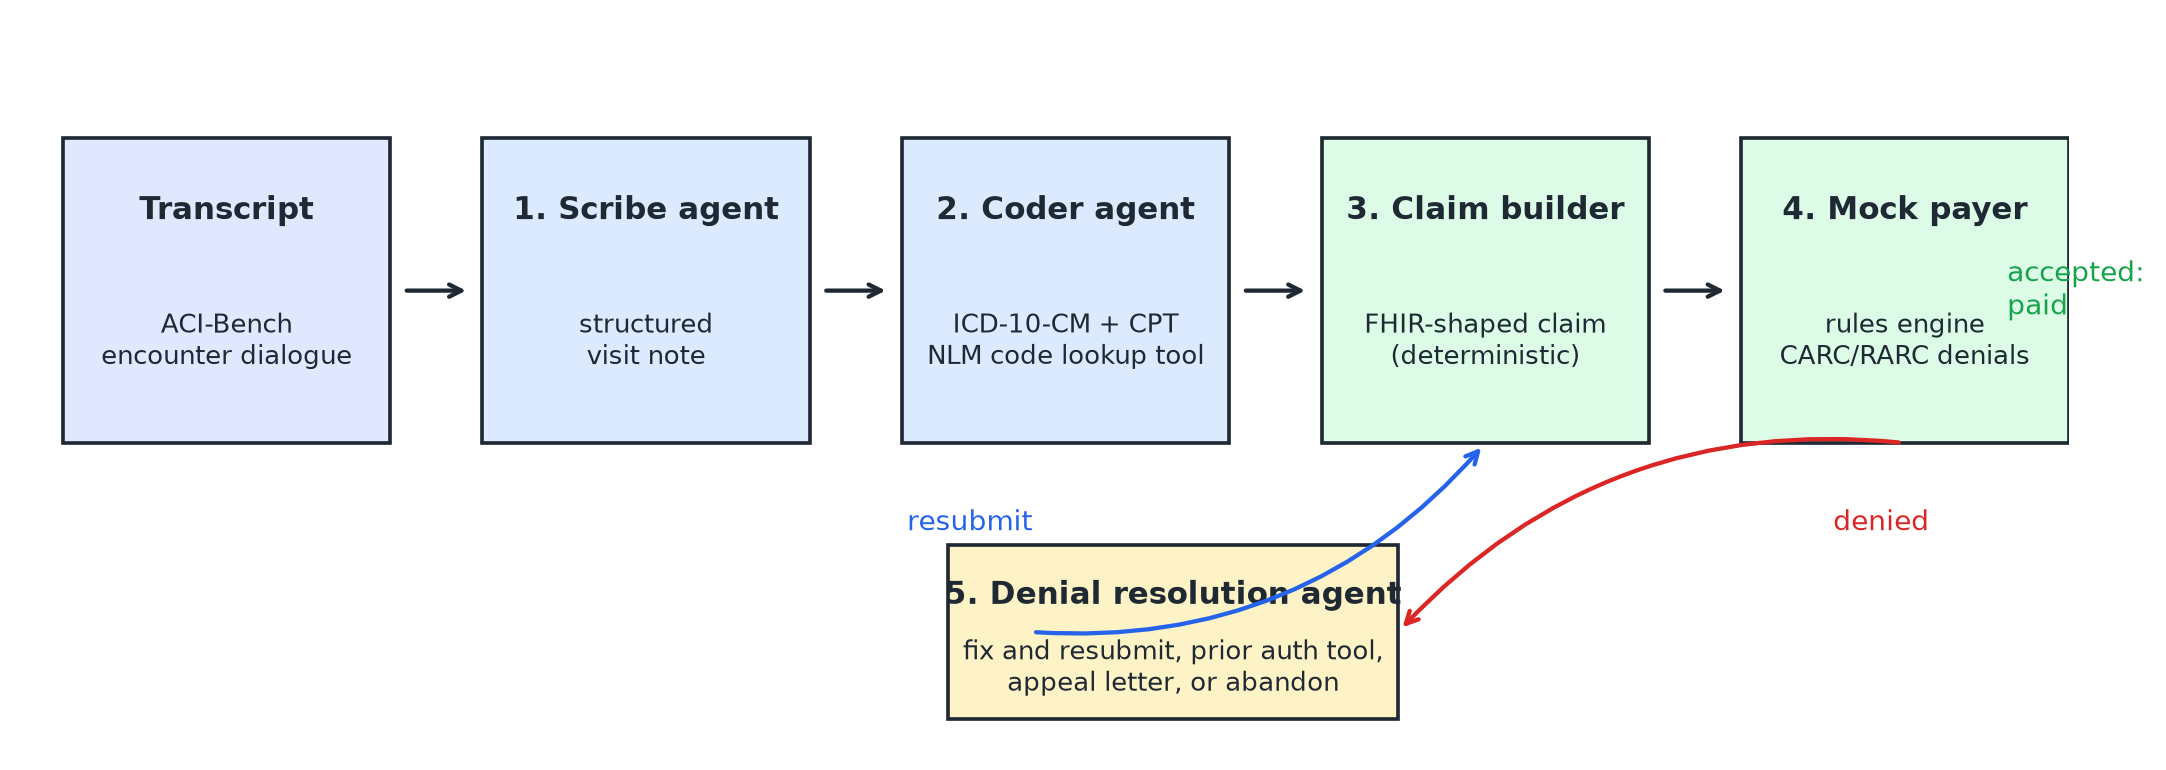
\includegraphics[width=0.95\textwidth]{figures/workflow.png}
  \caption{The ClaimLoop pipeline. Stages 1, 2, and 5 are LLM agents; the
  claim builder and the payer are deterministic code. A denial routes the
  claim to the resolution agent, which can fix and resubmit (at most three
  submissions), request prior authorization through a portal tool, appeal in
  writing, or abandon.}
  \label{fig:workflow}
\end{figure*}

\textbf{Stage 1, scribe agent.} Receives the raw transcript and emits a
structured visit note (chief complaint, HPI, history, medications, allergies,
exam, results, per-problem assessment and plan, follow-up) as a typed schema.
Instructions forbid inventing information; absent sections are recorded as
not documented.

\textbf{Stage 2, coder agent.} Receives the note, not the transcript,
mirroring real coding workflows. It proposes ICD-10-CM diagnoses and must
verify every code through a search tool backed by the NLM Clinical Tables
API; unverified codes are not allowed into the output. Procedure codes are
restricted to a small demonstration fee schedule because the full CPT code
set is copyrighted by the American Medical Association and cannot ship with
an open repository; the schedule covers common evaluation and management,
imaging, injection, and laboratory codes matching the corpus specialties.
Each code carries a rationale, linked diagnosis pointers, and a confidence
estimate.

\textbf{Stage 3, claim builder.} Deterministic assembly of a FHIR-shaped
claim: patient and provider blocks, diagnosis list, service lines with
charges from the fee schedule, and any prior authorization numbers obtained
in earlier attempts. The builder intentionally does not second-guess the
coder; bad codes flow through so the payer can catch them.

\textbf{Stage 4, mock payer.} A rules engine, not a model. Table~\ref{tab:rules}
lists the rules and the public CARC codes they emit. Determinism matters
methodologically: identical claims receive identical verdicts, so any change
in outcome is attributable to the agent's revisions, and the evaluation can
report recovery rates per denial category. An unchanged resubmission is
denied as a duplicate, which prevents the degenerate strategy of simply
retrying.

\begin{table}
  \caption{Mock payer rules and their denial codes. Necessity and
  documentation thresholds are an illustrative demo policy, not any real
  payer's policy.}
  \label{tab:rules}
  \begin{tabular}{lll}
    \toprule
    Rule & CARC & Meaning \\
    \midrule
    Required fields present & CO-16 & claim lacks information \\
    Diagnosis code exists (NLM check) & CO-146 & invalid diagnosis \\
    Procedure on fee schedule & CO-181 & invalid procedure \\
    Valid diagnosis pointers & CO-16 & missing diagnosis link \\
    Necessity: dx supports procedure & CO-50 & not medically necessary \\
    Prior authorization on file & CO-197 & authorization absent \\
    High E/M level documentation & CO-150 & level not supported \\
    Changed claim on resubmission & CO-18 & duplicate claim \\
    \bottomrule
  \end{tabular}
\end{table}

\textbf{Stage 5, denial resolution agent.} Receives the note, the billed
coding, the claim, and the adjudication with CARC/RARC reasons, and chooses
to fix and resubmit, obtain prior authorization through a portal tool
(granted deterministically when the payer's own necessity policy is met),
write a first-level appeal letter, or abandon. Instructions prohibit
inventing clinical facts and prohibit upcoding; appeals are reviewed by the
payer against the full documented diagnosis list, modeling a human reviewer
reading the whole record.

\subsection{Evaluation design}
Each encounter is scored on workflow outcomes: whether the first claim was
accepted, whether a denied claim was eventually paid within three
submissions, which CARC categories appeared and which were successfully
resolved, and appeal outcomes. Note quality is scored as ROUGE-1/2/L against
the ACI-Bench reference note, connecting this work to the corpus's original
task. Cost is reported as tokens and wall time per stage. What is
deliberately not claimed is clinical coding correctness: ACI-Bench carries no
billing ground truth and I am not a certified coder, so code choices are
evaluated for schema validity, verifiability, and payer acceptance, not for
audit-grade accuracy. This boundary is stated because it is exactly where a
production system would insert human review.

\subsection{Implementation and reproducibility}
The pipeline is roughly two thousand lines of Python and JavaScript: a
FastAPI backend, three agents on the OpenAI Agents SDK (gpt-5.6 family
models, configurable effort), a React timeline frontend that renders every
artifact of the claim journey, and a pytest suite covering the payer rules.
Reproducibility levers: the dataset is fetched at a pinned commit, demo
identifiers are deterministic functions of the encounter id, the service
date is fixed, the payer is seedless and rule-based, and every evaluation
writes its exact configuration to results/eval\_config.json. The repository
contains no dataset text, per course rules and the corpus license.

\section{Results}

[RESULTS-PENDING: this section is populated from results/summary.json after
the evaluation batch. Planned content: (1) headline outcome funnel figure,
first-pass acceptance versus recovered versus unresolved; (2) denials by
CARC with recovery rates, Figure denials\_by\_carc; (3) a walkthrough of one
representative denial-recovery trajectory including the appeal letter; (4)
note quality ROUGE table against the ACI-Bench reference notes; (5) token
and latency table per stage and model tier; (6) failure taxonomy: which
denial categories resisted automation and why.]

\section{Limitations and Ethical Considerations}

The payer is a simulation with an intentionally small rule set; real
adjudication involves eligibility, bundling edits, timely filing, and
payer-specific medical policies that this demo does not model. The fee
schedule is a tiny paraphrased subset because CPT is AMA-copyrighted. The
corpus is simulated dialogue, which is what makes an open, PHI-free demo
possible, but it also means no claim about real-world performance is made.
Coding correctness is not clinically validated, and the system is presented
strictly as a research and teaching artifact, not billing advice or a
compliance tool. No real patient data was used at any point, no model was
fine-tuned, and the dataset is not redistributed.

\section{Conclusion}

ClaimLoop set out to test whether a small, readable stack of tool-using LLM
agents can carry an outpatient encounter through the full claims lifecycle,
including the part practitioners dread: the denial loop.
[CONCLUSION-PENDING: one paragraph summarizing what the numbers showed about
first-pass quality versus loop recovery, and the standout failure modes.]
Beyond the numbers, the project argues for a methodological pattern: when
studying agent behavior in administrative workflows, replace the opaque
counterpart (here, the payer) with a transparent deterministic environment,
and the agent's competence becomes measurable per failure category. Future
work: richer payer policies (bundling edits, eligibility), a human-in-the-loop
review queue, real 837/835 transaction formats, comparing model tiers and
effort settings on recovery rate, and testing whether the resolution agent's
appeal letters survive review by human billing professionals.

\bibliographystyle{ACM-Reference-Format}
\bibliography{claimloop}

\end{document}
